%
% This is LaTeX source for the scllmk logo.
%
% Copyright (c) 2018 Takayuki YATO (aka. "ZR")
%   GitHub:   https://github.com/zr-tex8r
%   Twitter:  @zr_tex8r
%
% The scllmk package is distributed under the MIT License.
%


% +++
% sequence = ["latex", "tex2img"]
%
% [programs.tex2img]
% command = "tex2img"
% opt = '--latex=lualatex --resolution=60 --margins "500 50"'
% arg = ["%T", "%B.png"]
% +++

\documentclass{article}

% ----- page size -----
\usepackage[paperheight=5.5cm, paperwidth=5.5cm]{geometry}

% ----- fonts -----
\usepackage{type1cm}
\newcommand{\mainfont}{\usefont{OT1}{cmfr}{m}{it}}
\newcommand{\subfont}{\usefont{OT1}{cmfr}{m}{n}}

% ----- colors -----
\usepackage{xcolor}
% paleturquoise (RGB: 169, 255, 242; CMYK: 23, 0, 12, 0)
\definecolor{color1}{RGB}{169, 255, 242}
% symphony blue (RGB: 24, 87, 227; CMYK: 92, 63, 0, 0)
\definecolor{color2}{RGB}{24, 87, 227}
% obaku (RGB: 255, 242, 127; CMYK: 1, 5, 62, 0)
\definecolor{color3}{RGB}{255, 242, 127}

% ----- tikz -----
\usepackage{tikz,scsnowman}
\usetikzlibrary{calc}

% ----- logo itself -----

\begin{document}

\thispagestyle{empty}

\centering
\null\vfill

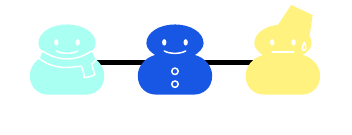
\begin{tikzpicture}[x=1pt,y=1pt]
\useasboundingbox
  (-14.22636,-14.22636) rectangle (92.6128,14.22636);
\draw [ultra thick] (0,1.6) -- (78,1.6);

\node at (0,6.6)
  {\scsnowman[scale=5,body=color1,muffler=color1]};
\node at (39,6.6)
  {\scsnowman[scale=5,body=color2,buttons=color2]};
\node at (78,6.6)
  {\scsnowman[scale=5,body=color3,hat=color3,
      sweat=color3,mouthshape=tight]};
\end{tikzpicture}

\vspace{0.25cm}

\sffamily
{\Huge\mainfont scllmk} \\
{\scriptsize\subfont SC Light {\LaTeX} Make}

\vfill

\end{document}
